\section{Automatic Plagiarism Detection Webservices}

Unplagged itself is a workbench, where the plagiairism detection is done by hand. Although it provides useful automatic tools that help the user to make the process of plagiairism detection easier. One of these tools are external webservices that check a specific text for plagiairism and try to find sources which can be used for further inspections.

We were talking to 3 companies offering such a webservice: Docoloc, PlagScan and PlagAware. As a proof of concept the PlagAware webservice has been implemented and added to our application, it will be described in the following section.

\subsection{PlagAware}

PlagAware, a website for automatic plagairism detection is a commercial website which costs money depending on the amount of text to analyze. It figures out possible sources of the text handed in on their website and creates a PDF report with a list of all the found sources (figure \ref{fig:plagaware-result}).

\begin{figure}[!h]
  \centering
  \fbox{
    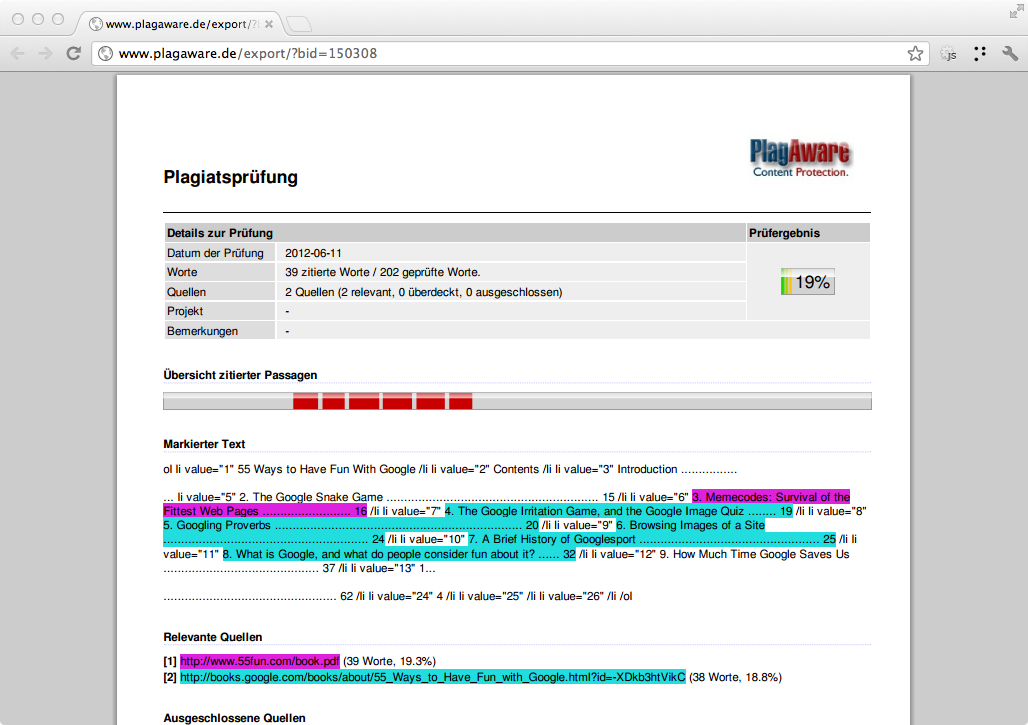
\includegraphics[width=0.97\textwidth]{images/feature-plagaware-result.png}
  }
  \caption{PlagAware result document}
  \label{fig:plagaware-result}
\end{figure}

The website also offers a webservice which takes text as input and notifies the user when the analyzing is finished. Although it does not provide any information about the sources through the webservice response call, there is only a status code and the percentage of plagairism responded. Whenever the response was sent, the user has to go to the PlagAware website and check out the detailed results there.

Since the PlagAware webservice is a simple HTTP-Webservice, the connection is done through an HTTP request with curl.
\begin{lstlisting}[caption=Sending a request through curl to the PlagAware webservice]
public function detect(Application_Model_Document_Page_DetectionReport &$report){
    $url = "http://www.plagaware.de/service/submittext";
    $fields = array(
      'UserCode'=>urlencode($this->paUserCode),
      'ResultUrl'=>urlencode($this->paResultUrl . $report->getId()),
      'TestText'=>urlencode($report->getPage()->getContent()),
      'DryRun'=>urlencode($this->paDryRun)
    );

    // url-ify the data for the POST
    $fields_string = "";
    foreach($fields as $key=>$value){
      $fields_string .= $key . '=' . $value . '&';
    }
    rtrim($fields_string, '&');

    $ch = curl_init();
    curl_setopt($ch, CURLOPT_URL, $url);
    curl_setopt($ch, CURLOPT_RETURNTRANSFER, 1);
    curl_setopt($ch, CURLOPT_CONNECTTIMEOUT, 10);
    curl_setopt($ch, CURLOPT_POST, count($fields));
    curl_setopt($ch, CURLOPT_POSTFIELDS, $fields_string);

    $output = curl_exec($ch);
    $info = curl_getinfo($ch);
    curl_close($ch);
}
\end{lstlisting}

The response is sent through a GET-Request to a pre-defined request URL, in our case '/document/response-plagiarism/report/<report-id>'. The call of this action stores the result in our database and creates a notifcation for the user, indicating that a new report is available.